\chapter{Interception HTTPS}

\label{sec:https-interception}

\begin{figure}[H]
  \caption{Attaque HTTPS interception (diagramme Dia)}
  \fbox{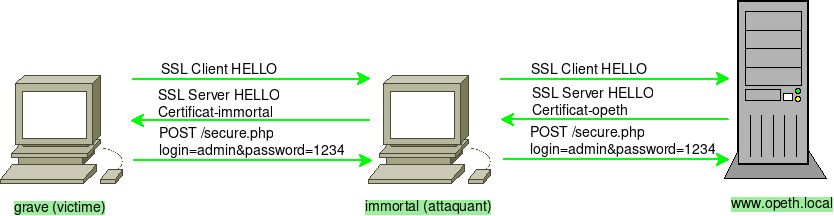
\includegraphics[width=\textwidth]{../medias/https-interception/attack.png}}
\end{figure}

La nouvelle méthode que nous allons voir pour intercepter un traffic https n'est pas vraiment une attaque. Pour être menée à bien, la machine placée en homme du milieu doit avoir installé sa propre authorité de certification, et surtout l'avoir rentrée sur la machine du client, en amont.

C'est une chose qui peut être assez dure à réaliser pour un attaquant, mais il y a des cas où cette situation se trouve. Dans le cadre d'une entreprise, il n'est pas rare que les requêtes http des employés passent par un proxy, pour suivre leur activité. Les responsables n'ont par contre, a priori pas moyen de lire les requêtes https. 

C'est en fait au contraire assez simple à réaliser dans la mesure où il est facile de rajouter une authorité de certification à la main dans les navigateurs web de tous les employés.

L'idée de la méthode est d'agir comme un simple proxy https. Lors de la connexion initiale du client vers le site web, la machine placée en homme du milieu va récupérer la requête, et établir elle même une connexion avec le serveur distant. Le proxy n'a plus qu'à établir une connexion avec le client, ce qui ne pose pas de problème car l'authorité de certification est acceptée par le navigateur du client.




